\documentclass[10pt,a4paper]{article}
\usepackage[utf8]{inputenc}
\usepackage{amsmath}
\usepackage{amsfonts}
\usepackage{amssymb}
\usepackage{graphics}
\usepackage[margin=1in]{geometry} 
\usepackage{amsmath,amsthm,amssymb,amsfonts}
 
\newenvironment{problem}[2][Problem]{\begin{trivlist}
\item[\hskip \labelsep {\bfseries #1}\hskip \labelsep {\bfseries #2.}]}{\end{trivlist}}
%If you want to title your bold things something different just make another thing exactly like this but replace "problem" with the name of the thing you want, like theorem or lemma or whatever

\begin{document}
\author{Peter Shaffery}
\title{Numerical Analysis II: Homework 7}
\maketitle
\section{Problems}
\begin{problem}{1}
Implement the trap rule with repeated Richardson extrapolation to numerically integrate the ODE $t^2 y'' + t y' + (t^2 - 1) y = 0$ with IC $y(0) = 0$ and $y'(0) = \frac{1}{2}$.
\end{problem}
Converting the given, second order ODE to a system of first-order ODEs is not entirely trivial.  If we naively set $x = y$ and $z = y'$ then we end up with the system:
\[
\begin{split}
x' &= z\\
z' &= - \left( \frac{1}{t} z + \left( 1-\frac{1}{t^2} \right) x \right)\\
\end{split}
\]
But since $z(0) = \frac{1}{2}$ the RHS of this system has a gaping singularity at the initial conditions. We could fudge the numerical integration a little, and start it \textit{close} to 0 (and I'm still going to end up doing that), but we should at least be circumspect about it to make sure that's rigorously justifiable.

To start let's say Taylor expand $y(t)$ with a twist, set $y(t) = \sum\limits_{n=0}^{\inf} a_n t^{n+r}$ where $r$ is a yet-to-be-determined constant.  Plugging this expansion into the ODE, simplifying some polynomial terms, and collecting terms with the same powers of $t$ gives us the following:
\begin{equation}
(r^2-1)a_0 t^r + r(2r+1) a_1 t^{r+1} + \sum\limits_{n=2}^{\inf} \left[ \left( (n+r)^2-1 \right) a_n + a_{n-2} \right] t^{n+r} = 0
\end{equation}

Since this is a polynomial in $t$ we know that it can be set to $0$ if all polynomial coefficients are $0$, so from (1) we get the following equalities:
\begin{equation}
\begin{split}
(r^2 - 1) a_0 &= 0\\
r(2r+1) a_1 &= 0\\
\left( (n+r)^2-1 \right) a_n + a_{n-2} &= 0\\
\end{split}
\end{equation}

From the third equality we have the recursion relation $a_n = -\frac{a_{n-2}}{(n+r)^2-1)}$ with $n=2,3,...$ and we will use the first two to determine $r$.  If we set $r= \pm 1$ then this solves the first one, but then if $r=-11$ our recursion relation has a singularity when $n=2$.  Let's sidestep this by setting $a_0 = 0$ (note that this is consistent with setting $r=1$, as doing so means that the modified Taylor expansion $y(t) = \sum\limits_{n=0}^{\inf} a_n t^{n+r}$ starts with the $t$ term, so the `true' Taylor series $y(t) = \sum\limits_{n=0}^{\inf} b_n t^n$ must have $b_0 = 0$).  Now we use the second equation to say that $r=0,\frac{-1}{2}$ which causes no problems with the recursion relation.  Not a useful fact here, but not that since $a_0$, then all $a_n =0$ when $n$ is even.

Letting $y_r(t) = \sum\limits_{n=0}^{\inf} a_n t^{n+r}$ then let's say that $y(t) = c_1 y_0(t) + c_2 y_{1/2}(t)$.  Since $y'(0) = \frac{1}{2}$, but $y'_{1/2}(t)$ doesn't converge when $t=0$ (the first term in the sum has a factor of $\frac{1}{\sqrt{t}}$, I'm going to say that $c_2 =0$ to match the IC.  Let's just assume then that $c_1 = 1$ and then use the IC to determine $a_1$ (the is basically just setting the expansion coefficients $a_n' = c_1 a_n$).  Note that $y'_0(0) = a_1$ so we have that $a_1 = \frac{1}{2}$, and now we can determine the rest of the odd $a_n$ from the recursion relation if we need (recall that $a_n = 0$ when $n$ is even).

Okay so at this point we're going to say that $y(t) = t u(t)$, so $u(t) = \sum\limits_{k=0}^{\inf} a_{2k+1} t^{2k}$.  Noting that $y' = u + t u'$ and since $y'' = 2u' + t u''$ we can plug these in to the original ODE and conclude that $t u'' + 3u' + tu =0$ so therefore $u'' + \frac{3}{t}  u' + u = 0 $.  We now have no problem with singularities since $u'(t) = 2 a_3 t + 4 a_5 t^3 +...$ so $\frac{1}{t} u'(t)= 2 a_3 + 4 a_5 t^2 + ...$ which is probably analytic.

Now let's reset all of our notation and pretend that we're starting fresh with the ODE $u'' + \frac{3}{t}  u' + u = 0 $ and IC $u(0) = \frac{1}{2}$ and $u'(0) = 0$.  Furthermore we're going to assume (based on the previous work) that the solution $u(t)$ is analytic.  Now even though the LHS of the ODE is undefined at $t=0$, we can basically start the integration at $t = \epsilon$ for any small, positive $\epsilon$ and feel comfortable that nothing weird is going to happen since we know that $\lim_{t \rightarrow 0} u(t) = \frac{1}{2}$ and $\lim_{t \rightarrow 0} u'(t) = 0$ and that (again from the previous work) the error incurred by doing so is pretty small (just look at the Taylor series and we can see that we're dealing with errors on the order of, like, $\epsilon$ or better.

Okay so now let's use the notation reset and set $x(t) = u(t)$ and $y(t) = u'(t)$, and define the vector $\vec{x}(t) = [x(t), y(t)]^T$.  Now we convert our second order ODE to the following first order, vector ODE:
\begin{equation}
\vec{x}' = \left[
\begin{array}{cc}
0 & 1\\
-1 & -3/t\\
\end{array}
\right]
 \vec{x} = A(t) \vec{x}
\end{equation}

This is very amenable to the trap rule for ODEs, which will be  of the form $\vec{x}_{n+1} = \vec{x}_{n} + \frac{h}{2} \left( A(t) \vec{x}_n + A(t) \vec{x}_{n+1} \right)$.  Therefore a forward step of this algorithm consists of just solving the system $(I - \frac{h}{2} A(t)) \vec{x}_{n+1} = v(t)$ where $v(t) = (I + \frac{h}{2} A(t)) \vec{x}_n$.  Once we have approximated $u(t)$ we can just multiply it by $t$ to get $y(t)$.

I performed the Repeated Richardson Extrapolation `passively'.  That is, I trap-integrated the ODE system for the $k$ user-chosen steps for $n$ different step sizes $h, 2^{-1} h,...,2^{-n} h$, and then pulled the integrated values at the time values $t_0, t_1 = t_0 + h, ..., t_k = t_0 + kh$.  For each $t_k$ I then evaluated a $n \times n$ Richardson Extrapolation table (see Dahlquist and Bjork diagram 7.2.13) using the estimated function value from each step-size at that time step and set my final function approximation $\hat{u}(t)$ equal the Richardson Extrapolated value.  This passive approach is contrasted with the active approach, which evaluates the $n \times n$ Richardson Extrapolation across the step-sizes at every time step, and then starts the next trap-integration step (for every step size) from the Richardson Extrapolated value, rather than at the previous value from the appropriate step size integration.

With $h=1e-5$ and $n=2$ I was able to achieve 6 decimal places of accuracy.  Increasing $n$ for this step size didn't seem to improve the accuracy and decreasing $h$ made the code run-time impractical.  I probably haven't implemented the Richardson Extrapolation correctly, or maybe my code has too much overhead, but at this point I've spent too much time with this problem to make further tweaks or improvements.  Fig. 1 plots my integrated values of $y(t)$ against SciPy's Bessel Function of the First Kind of Order 1 (although the 6 decimal accuracy is really visible from this plot).  See Appendix for code.

\begin{figure}
\centering
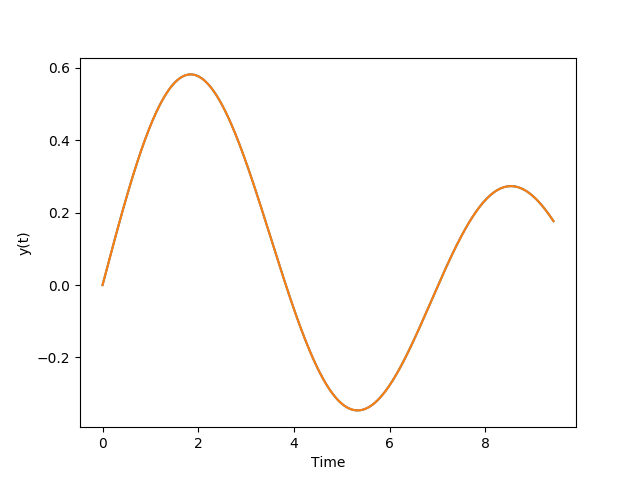
\includegraphics{./Figs/plot.png}
\caption{Integrated Solution plotted over True Solution}
\end{figure}

\begin{problem}{2}
Show that the two-step method $y_{n+1} = \frac{1}{2}(y_n + y_{n-1}) + \frac{h}{4}[4f(x_{n+1},y_{n+1}) - f(x_n,y_n) + 3 f(x_{n-1}, y_{n-1})]$ is second order.
\end{problem}
\begin{proof}
  This is a quick application of Izerles Thm 2.1.  Following the notation of the theorem, note that $\rho(w) =  w^2 - \frac{1}{2} w - \frac{1}{2}$ and that $\sigma(w) = w^2 - \frac{1}{4} w + \frac{3}{4}$.  To show that the method is of order 2, then we need to show that $\rho(e^h) + h \sigma(e^h) = \mathcal{O}(h^3)$ (by the proof of Thm 2.1 this is an equivalent formulation to how the theorem is `officially' presented).  Plugging this expression into Mathematica and using the \textit{Series[]} function on $\rho(e^h) + h \sigma(e^h)$ expanding in terms of $h$ about $h=0$ to $5^{\text{th}}$ gives that $\rho(e^h) + h \sigma(e^h) = \frac{-5}{8} h^3 + \mathcal{O}(h^4)$, hence the method is of order 2.
\end{proof}

\begin{problem}{3}
Determine the order of the method $y_{n+1}  = 4 y_n - 3 y_{n-1} - 2h f(x_{n-1}, y_{n-1})$ and illustrate with an example that the method is unstable.
\end{problem}
\begin{proof}
So again we set $\rho(w) = w^2 - w + \frac{3}{4}$ and $\sigma(w) = -2$ and use the Mathematica \textit{Series[]} function to determine that the series of expansion of $\rho(e^h) - h \sigma(e^h) = -\frac{3}{4} + \mathcal{O}(h)$ which is pretty bad.

To show that it was unstable I did a quick implementation of this algorithm on the ODE $y'=-y$ (which has exact solution $y(t) = e^{-t}$) .  I chose $h = 1e-5$, $t_0 =0$ and started the algorithm with $y_0 = 1$ and $y_1 = e^{-h}$.  After 101 iterations I had $y_{101} = 2.7e32$, with the true solution $y(101*h) \approx 0.998$ and decreasing. 
\end{proof}

\begin{problem}{3}
Show that the multistep method $y_{n+3} + a_2 y_{n+2} + a_1 y_{n+1} + a_0 y_n = h[b_2 f(t_{n+2},y_{n+2}) + b_1 f(t_{n+1},y_{n+1}) + b_0 f(t_n,y_n)$ is fourth order iff $a_0 + a_2 = 8$ and $a_1 = -9$.  Deduce that this method cannot be both fourth order and convergent.
\end{problem}
\begin{proof}
Since $\rho(w) = w^3 + a_2 w^2 + a_1 w + a_0$ and $\sigma(w) = b_2 w^2 + b_1 w^2 + b_0$, then from Mathematica we have that if the method is fourth order the following set of equations must be satisfied (found by taking the Taylor expansion and setting all coefficient of $h^k$ to 0 for $k=0,1,2,3,4$):
\begin{equation}
\begin{split}
1 + a_0 + a_1 + a_2 &= 0\\
3 + a_1 + 2 a_2 - b_0 - b_1 - b_2 &= 0\\
9 + a_1 + 4 a_2 - 2 b_1 -4 b_2 &= 0\\
27 + a_1 + 8 a_2 - 3 b_1 -12 b_2 &=0\\
81 a_1 + 16 a_2 - 4 b_1 -32 b_2 &= 0\\
\end{split}
\end{equation}
This is five equations for six variables, so that explains why we have that $a_0$ and $a_2$ must lie on a line.  Furthermore, the first condition requires $a_0 + a_1 + a_2 = 1$, so if $a_1 = -9$ then we have also that $a_0 + a_2 = 8$.

This equations can be solved simultaneously using your favorite method (the best way would probably be to put them into matrix form and then Gauss-Jordan reduce, but I just used Mathematica's \textit{Solve[]} function) to determine that they are satisfied if $a_1 = -9, a_2 = 8-a_0, b_0 = \frac{1-a_0}{3}, b_1 = \frac{14-4a_0}{3}, \text{ and } b_2 = \frac{17 - a_0}{3}$, which gives the first result we wanted, namely that the method is fourth order if $a_1 = -9$ (and therefore $a_0 + a_2 = 8$).

Now assume the method is fourth order, ie. $a_1 = -9$ and $a_0 + a_2 = 8$.  The first characteristic polynomial is then $\rho(w) = w^3 + (8-a_0) w^2 - 9 w + a_0$.  Using \textit{Solve[]} we have that $\rho(w)$ has three roots, a simple root at $w_0=1$ and then two roots $w_{1,2} = \frac{1}{2} \left( -9 + a_0 \pm \sqrt{81 - 14 a_0 + a_0^2} \right)$ (assuming that $a_0$ is real).

Now note that if $w_1$ is complex then so is $w_2$ and that furthermore they have the same modulus.  This requires that $81 - 14 a_0 - a_0^2 <0$, but a quick analysis of the polynomial on the LHS of this inequality indicates that it is strictly positive for real $a$ (both its roots are complex and it is positive for $a_0 =1$, hence it is positive everywhere).  Therefore $w_1$ and $w_2$ are both real for real $a_0$.

Next we note that $w_1 - w_2 = \sqrt{81 - 14 a_0 + a_0^2}$.  The minimum value of $81 - 14 a_0 + a_0^2$ occurs for $-14 + 2 a_0 =0$ or $a_0 = 7$.  However this means that $\min_{a_0} [w_1(a_0) - w_2(a_0)] = \sqrt{81 - 14*7+7^2} = 4 \sqrt{2}$.  Hence even if one of the roots is within the unit disk in the complex plane, the other cannot be since the distance between then excedes the radius of the circle.

Since $\rho(w)$ cannot satisy the root condition if $a_0 + a_2 = 8$ and $a_1 = -9$, and this is the only time that the method is fourth order we conclude that the method cannot be be both fourth order and convergent.
\end{proof}

\section{Appendix: Code}
\begin{verbatim}
import numpy as np
import scipy as sp
import scipy.optimize as spot
import numpy.linalg as npla
import matplotlib.pyplot as plt
from tqdm import *

class ode_obliterator_v2(dict):
    def __init__(self, RHS, init_val, init_time=0, h=1e-1, q=2,n=2):
        self.yp = RHS
        self.iv = np.array(init_val)
        self.init_time = init_time
        self.t = init_time
        self.h = h
        self.q = q
        self.n = n
        self.dim = max(self.iv.shape)

        self.sol = self.iv
        self.times = np.array([self.t])

	#Forward step of the trap rule
    def sacramento_scramble(self,h,curr,t):
        v = curr + .5*h*np.dot(self.yp(t),curr)
        A = np.eye(self.dim) - .5*h*self.yp(t+h)
        output = npla.solve(A,v)
        return(output)
        
    #Richardson Extrapolation using table method
    def boston_u_turn(self,init):
        n = len(init)
        table = np.zeros([n,n])
        table[:,0] = init

        for j in range(1,n):
            for i in range(j,n):
                p = 2*j+1
                table[i,j] = table[i,j-1] +(table[i,j-1] - table[i-1,j-1])/float(self.q**p-1) 

        update = table[n-1,n-1]

        return(update)
	#Trap integrate for multiple step sizes
    def boulder_shimmy(self,end_time):
        t_steps = np.arange(self.init_time,end_time,self.h)
        self.multigrid = np.zeros([self.n,len(t_steps),self.dim])
        for k in range(0,self.n):
            h = self.q**(-1*k)*self.h
            curr = self.iv
            for t in tqdm(range(len(t_steps))):
                time = t_steps[t]
                for i in np.arange(self.q**k):
                    curr = self.sacramento_scramble(h,curr,time)
                    time += h
                
                self.multigrid[k,t,:] = curr
    
    #Take multiple integrations with different step sizes and perform 
    #Richardson extrapolation to get the final result    
    def houston_plug_n_chug(self,end_time):
        self.boulder_shimmy(end_time)
        hold = np.zeros(self.multigrid.shape[1:3])
        for i in tqdm(range(hold.shape[0])):
            for j in range(hold.shape[1]):
                hold[i,j] = self.boston_u_turn(self.multigrid[:,i,j])

        self.sol = hold
        self.times = np.arange(self.init_time,end_time,self.h)

    
def ode(t):
    A = np.array([[0.,1.],[-1.,-3./t]])
    return(A)

y0 = np.array([.5,0.])
trap_solve = ode_obliterator_v2(ode,y0, init_time = 1e-10, h = 1e-5,n=2)
trap_solve.houston_plug_n_chug(3*np.pi)

x = trap_solve.times
y_true = sp.special.jv(1,x)
y_int = x*trap_solve.sol[:,0]

err = max(y_int-y_true)

plt.plot(x,y_true)
plt.plot(x,y_int)
plt.show()

\end{verbatim}

\end{document}

%%% Local Variables:
%%% mode: latex
%%% TeX-master: t
%%% End:
